\documentclass[a4paper, 10pt,onecolumn]{scrartcl}
\usepackage[ngerman]{babel}
\usepackage[T1]{fontenc}
\usepackage[utf8]{inputenc}
\usepackage{multirow}
\usepackage{natbib}
\usepackage{graphicx}
\usepackage{amsmath, amssymb}
\usepackage{graphicx}
\usepackage{grffile} %einfacheres einbinden von Dateipfaden
\usepackage{xpatch} %more space between title and subtitle
\usepackage{mathtools}

\newlength{\myspace}
\setlength{\myspace}{2em}

\makeatletter
\xpatchcmd{\@maketitle}{\vskip.5em}{\vskip\myspace}{}{}
\makeatother



\title{Computationalphysics 1: Übungsaufgabe Numerische Integration} 
\subtitle{Aufgabe 1: Konvergenz des Rechteckverfahrens}
\author{Jakob Hollweck} %auch nach \begindocument möglich
\setlength{\parindent}{0pt}
\date{Abgabe 17.11.17}

\begin{document}
\maketitle


\section{Differenz Numerisches Ergebnis - Analytisches Ergebnis}



\begin{figure}[ht!]
	\centering
	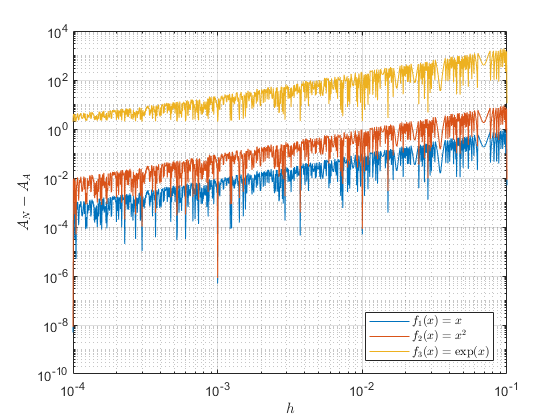
\includegraphics[scale=0.5]{Diffs.png}
	\caption{$A_N - A_A$ über $h$} 
	\label{Abbildung1}
\end{figure}

Das erarbeitete Skript zur numerischen Integration basierend auf der Rechteckregel liefert für die Berechnung der Differenz des numerischen und analytischen Ergebnisses für $f_1(x)=x$, $f_2(x)=x^2$ und $f_3(x)=\exp(x)$ auf dem Intervall [0,10] und der Schrittweite $h \in [10^{-4},10^{-1}]$, die in Abbildung \ref{Abbildung1} aufgezeigten Graphen. 
Es ist zu erkennen, dass die Differenzen zwischen numerischem und analytischem Integral mit steigendem $h$ linear zunehmen. Dies bestätigt die Vorlesung, die hierfür das Verschwinden der ungeraden Terme der Taylorentwicklung bei der Integration über die Teilintervalle als Erklärung anbringt. 


\section{Stammfunktionen für verschiedene Startpunkte}


\begin{figure}[ht!]
	\centering
	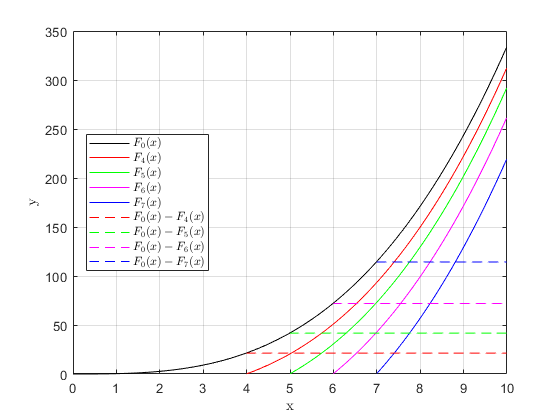
\includegraphics[scale=0.5]{Fs.png}
	\caption{Stammfunktionen $F_a(x)$ von $f(x)=x^2$ für verschiedene Startpunkte $a$}
	\label{Abbildung2}
\end{figure}

Des weiteren wurde untersucht, inwiefern das numerische Integral der Funktion $f(x)=x^2$ von der Wahl des Startpunktes $a$ abhängt. Abbildung \ref{Abbildung2} zeigt, dass die Wahl der Integrationsmethode dazu führte, dass nur noch langsam veränderliche Funktionen gut approximiert werden können. Der Graph zeigt, dass für größer werdende $a$ die Qualität der Approximation abnimmt. Der Grund hierfür ist, dass größere $a$ auch eine größere Änderung der Stammfunktion an dieser Stelle bedeuten. Dies wurde durch Differenzen der einzelnen Stammfunktionen deutlich gemacht. Dies ist auch in Abbildung \ref{Abbildung1} zu sehen, da die Funktion mit dem größten Anstieg auch den größten Fehler liefert.

\end{document}